\documentclass[letter, 10pt]{article}
\usepackage[utf8]{inputenc}
\usepackage[spanish]{babel}
\usepackage{amsfonts}
\usepackage{amsmath}
\usepackage{graphicx}
\usepackage{multirow}
\usepackage{enumerate}
\usepackage{listings}
\usepackage{url}
\usepackage{mathtools}
\usepackage[top=3cm,bottom=3cm,left=3.5cm,right=3.5cm,footskip=1.5cm,headheight=1.5cm,headsep=.5cm,textheight=3cm]{geometry}

\begin{document}
\title{Inteligencia Artificial \\ \begin{Large}Informe Final:
	 \textit{Green Vehicle Routing Problem (G-VRP)}\end{Large}}
\author{Felipe Chacón Ossa}
\date{\today}
\maketitle

%--------------------No borrar esta secci\'on--------------------------------%
\section*{Evaluaci\'on}

\begin{tabular}{ll}
Mejoras 1ra Entrega (10 \%): &  \underline{\hspace{2cm}}\\
C\'odigo Fuente (10 \%): &  \underline{\hspace{2cm}}\\
Representaci\'on (15 \%):  & \underline{\hspace{2cm}} \\
Descripci\'on del algoritmo (20 \%):  & \underline{\hspace{2cm}} \\
Experimentos (10 \%):  & \underline{\hspace{2cm}} \\
Resultados (10 \%):  & \underline{\hspace{2cm}} \\
Conclusiones (20 \%): &  \underline{\hspace{2cm}}\\
Bibliograf\'ia (5 \%): & \underline{\hspace{2cm}}\\
 &  \\
\textbf{Nota Final (100)}:   & \underline{\hspace{2cm}}
\end{tabular}
%---------------------------------------------------------------------------%
\vspace{2cm}

\begin{abstract}
En el presente informe se abordará el problema \textit{Green Vehicle Routing Problem} \textbf{G-VRP}, el cual consiste en optimizar la distancia total que recorre una flota de vehículos, cuyo combustible utilizado es ecológico, por lo tanto, tiene más restricciones en cuanto a la recarga del combustible. 
Además, dentro del estado del arte del problema, se podrán observar problemas similares al \textit{G-VRP} y otras variantes del mismo,
como el \textit{E-VRPTW}, \textit{RVRP}, entre otros, junto con
las técnicas utilizadas en ellos. También, habrá una descripción de las heurísticas utilizadas para
resolver instancias en el paper que presentó el problema junto con algunos resultados de
aplicarlas a instancias. 
También se verá su formulación matemática que incluye la función objetivo y las restricciones con sus
respectivas descripciones. 

\end{abstract}

\section{Introducci\'on}
El \textit{Green Vehicle Routing Problem} surge de la necesidad de ayudar a organizaciones públicas y privadas que buscan utilizar, en algún grado de proporción, vehículos con combustibles menos dañinos para el medio ambiente como podría ser el biodiesel, el gas natural líquido o el gas natural comprimido \cite{E-VRPTW}, pues estaciones de combustible
con la maquinaria necesaria para recargar este tipo de combustible son escasas \cite{G-VRP}, por lo que se plantea un modelo que permite abastecer eficientemente a lo largo de una ruta los vehículos.

El \textit{G-VRP}\cite{G-VRP}, como muchos problemas \textit{VRP}, es modelado como un grafo completo donde el objetivo consiste en minimizar la distancia de una flota de vehículos, que usan un tipo especial de combustible, los cuales salen desde un sitio, comúnmente conocido como almacén, para luego visitar a todos los clientes y, si fuera necesario, reabastecer su cantidad de combustible en algún momento de la ruta en lugares especiales destinados para ello, finalmente, luego de visitar todos los nodos clientes, debe volver al punto de partida, es decir, el almacén. Los arcos del grafo además de la distancia, poseen parámetros de costo de combustible y el tiempo que se demora un vehículo en recorrerlo.

Las autoras propusieron el problema para hacer más viable el uso de combustibles ecológicos dado el limitado número de estaciones que operan este tipo de combustible \cite{AFVs}, de esta forma, se piensa obtener recorridos óptimos considerando la necesidad de parar en estos puntos de recarga antes de quedar varados por la falta de combustible. Específicamente se refieren a los camiones que es el tipo de vehículo que más ha aumentado durante los últimos años, por lo tanto, al tener la viabilidad de cambiar a un combustible más amigable con el medio ambiente, se estará limitando la contaminación por dióxido de carbono. 

Este documento tiene por propósito entregar una descripción del problema junto con su
importancia, además, desarrollar una técnica para resolver las instancias del problema y analizar los resultados. Una descripción más detallada de las secciones se encuentra a continuación:

En la siguiente sección será descrito el problema con sus variables y las restricciones más importantes.
En la sección 3 se verá el estado del arte, presentando el origen y los motivos del problema junto a su importancia,
también serán detalladas las heurísticas usadas para llegar a soluciones cercanas a las óptimas, donde se
presentarán tablas con los resultados de ellas y se compararan. Luego, se describirán variantes 
del problema y contextos similares que desarrollan sus propias técnicas
y heurísticas acorde al tipo de problema.
En la sección 4 estará el modelo matemático del \textit{G-VRP} con la función objetivo y sus restricciones, todas con su
respectiva explicación.
Finalmente, en la sección 5 se presentan las conclusiones del informe.

\section{Definici\'on del Problema}
De acuerdo a \cite{G-VRP}, el problema busca encontrar a lo más \(m\) tours, uno por cada vehículo de una flota de vehículos que, partiendo de un nodo inicial, deben pasar por un conjunto de clientes, donde cada cliente es visitado por 1 solo vehículo y 1 sola vez, finalmente deben volver al punto inicial, en el que la suma total de la distancia de los tours es minimizada.
Cada vehículo cuenta con una restricción de distancia que puede recorrer en base a la cantidad de combustible que tiene,
como también existe una restricción de tiempo máximo para cada uno de los tours.

El G-VRP es definido como un grafo completo y no dirigido, donde los nodos se componen de los clientes, las estaciones de abastecimiento y el nodo inicial o almacén.
En cuanto a los arcos del grafo, al ser completo, cada nodo está conectado con todos los otros y cada arco tiene asociado parámetros, los cuales son el tiempo de viaje, el costo de combustible y la distancia hacia el nodo destino.
\bigskip

\textbf{Consideraciones adicionales son tomadas en cuenta}:
\begin{itemize}
\item Es posible recargar combustible en el almacén.
\item Se asume la misma velocidad para cada vehículo, la cual es constante.
\item Un vehículo puede recargar combustible las veces que sea necesario, pudiendo visitar más de 1 vez la misma estación de abastecimiento.
\item Cuando un vehículo llega a una estación de abastecimiento, es recargado hasta que el tanque esté lleno.
\end{itemize}

\textbf{Variables del problema}:
\begin{itemize}
\item La ruta que sigue cada vehículo.
\item La cantidad de combustible en el tanque del vehículo al visitar un cliente o
	una estación, o el mismo almacén.
\item La cantidad de tiempo total transcurrido de la flota al visitar un cliente, una estación o
	el almacén.
\end{itemize}

\textbf{Restricciones}
\begin{itemize}
\item Un vehículo no puede ir a un nodo al cual no tiene el combustible necesario para llegar.
\item El tour de un vehículo no puede superar un tiempo máximo.
\item Cada cliente es visitado solo una vez.
\item Todos los vehículos deben volver al punto de partida, es decir, el almacén.
\end{itemize}

\textit{G-VRP} es una variante del \textit{Vehicle Routing Problem (VRP)}\cite{VRP},
 problema que fue presentado en 1959, en él, solo se busca minimizar la distancia requerida para visitar cada cliente exactamente una vez sin restricciones de capacidad de combustible.

Anterior al \textit{G-VRP} está el \textit{Recharging Vehicle Routing Problem (RVRP)} que
utiliza nodos cliente como punto de abastecimiento, a diferencia del \textit{G-VRP} que tiene
puntos designados solo para la recarga del combustible y no corresponden a clientes. 
Existen otras variaciones que toman como base el \textit{G-VRP}, 
pues fue el primer problema en utilizar
estaciones de abastecimiento en vez de los nodos clientes, algunos ejemplos son 
\textit{Electric Vehicle Routing Problem with Time Windows and Recharging Stations (E-VRPTW)}, en el cual se puede realizar recargas parciales, las cuales tienen asociadas tiempos de recarga; y
\textit{G-VRP with Multiple Technologies and Partial Recharges (GVRP-MTPR)}, el cual,
además de las recargas parciales en \textit{E-VRPTW}, existen distintos métodos de recarga, los que
se diferencian en eficiencia y en tiempo que demora en recargar.

\section{Estado del Arte}

\subsection{G-VRP}
\textit{G-VRP} es una variante del \textit{VRP}, un problema que fue introducido por Dantzig y Ramser (1959), pero cuyas técnicas no
puede ser utilizadas, puesto que en \textit{G-VRP} las limitantes del combustible de cada vehícule indican donde poder viajar
o cuando reabastecerse de combustible. Siendo un problema relativamente nuevo, fue presentado por
 Erdogan y Miller-Hooks (2012), a la fecha de su publicación, no existían 
 variaciones de \textit{VRP} que fueran muy similares a \textit{G-VRP}, por lo que se
trabajó en heurísticas y métodos que resolvieran el problema en un tiempo viable.

A continuación, se explican las heurísticas utilizadas para \textit{G-VRP}:

\begin{itemize}
\item \textit{Modified Clarke and Wright Savings Algorithm (MCWS)}

Pasos:
	\begin{enumerate}
	\item Crear \(n\) tours de ida y vuelta, partiendo y finalizando en el almacén visitando un nodo cliente en el medio,
	 \(v_0 - v_i - v_0\) y agregarlo a una \textit{tours list}.
	 \item Calcular la duración y la distancia de cada tour en la \textit{tours list} y verificar su factibilidad,
	 	los tours que son posibles van a una \textit{feasible tours list} y los que no
	 	a una \textit{infeasible tours list}.
	 \item Por cada tour en la \textit{infeasible tours list} agregar el nodo de abastecimiento con el menor costo, el
	 que esta dado por \(c(v_i,v_0) = d(v_i, v_f) + d(v_f, v_0) - d(v_i,v_0)\), donde \(v_f\) es un nodo de
	  abastecimiento. Si el nuevo tour cumple las limitantes de distancia y tiempo, se agrega a la \textit{feasible tours list}, si no, se descarta el nuevo tour.
	  \item Calcular la ganancia al unir cada par de tour en la \textit{feasible tours list} con la condición que
	  cada par de nodos se encuentran en diferentes tours, la ganancia esta dada por
	  \(s(v_i,v_j) = d(v_0,v_i) + d(v_0, v_j) - d(v_i, v_j)\), la cual es guardada en una
	   \textit{savings pair list (SPL)} y ordenada de manera descendente.
	   \item Mientras la \textit{SPL} no esté vacía, se selecciona el primer par de nodos \(v_i, v_j\)
	   y se mezclan sus respectivos
	   tours, se revisa si cumple las limitantes de distancia y de tiempo, si cumple, entonces se agregan a
	   la \textit{feasible tours list}, si falla solo la restricción de distancia, se calcula el costo de agregar
	   un nodo de abastecimiento \(c(v_i,v_j) = d(v_i, v_f) + d(v_f, v_j) - d(v_i,v_0) - d(v_j,v_0)\) para el par
	   \(v_i,v_j\) y se agrega el que tenga el menor costo para el cual sea factible el tour. Si el tour resultante
	   tiene más de un nodo de abastecimiento, se revisa si es posible sacar uno o más de ellos. Finalmente el tour
	   resultante es agregado a la \textit{feasible tours list}.
	   Si fue agregado algún tour, se vuelve al paso 4, si no, se termina la heurística.
	\end{enumerate}
	
	Finalmente, con los tours en la \textit{feasible tours list}, tenemos una solución para el problema, donde la 
	cantidad de tours requeridos puede ser menor a la cantidad de vehículos disponibles, lo cual no produce problemas,
	sin embargo, si la cantidad de tours es mayor, será necesario tener más vehículos a disposición.
	
	Parte del proceso que realiza \textit{MCWS} es explicado a continuación:
	
	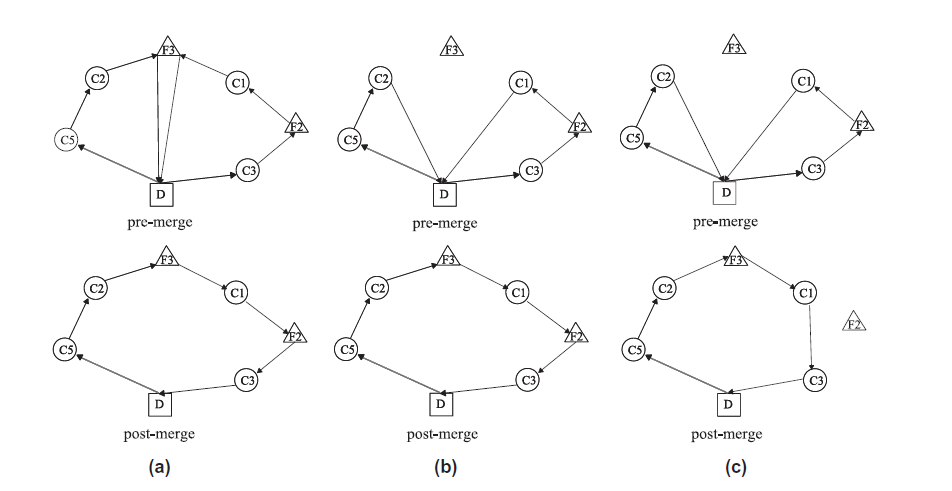
\includegraphics[width=1\textwidth]{mcws.PNG}
	
	Se pueden observar 2 tours con redundancia en la primera imagen de la parte superior,
	 es decir, que visita dos puntos de abastecimiento
	innecesariamente, la heurística elimina la redundacia y minimiza la distancia recorrida, luego
	se mezclan estos dos tours como se ve en la primera imagen de la sección inferior, al igual que antes,
	se encuentra redundacia, pues se visita \(F3\) y \(F2\), la heurística prueba sacando uno de los nodos de 
	abastecimiento encontrando un tour factible que utiliza menor distancia, el cual es agregado
	 a la \textit{feasible tours list}.
	 
\item \textit{The Density-Based Clustering Algorithm (DBCA)}

Esta heurística está pensada para aprovechar la característica espacial del problema, \textit{DBCA} es una
técnica de \textit{clustering} y descompone el problema en subproblemas.

Para cada nodo en el grafo, se revisa su vecindad con un radio de largo \(\varepsilon\) y debe contener
un mínimo de vecinos \textit{minPts} para ser considerado núcleo del cluster. 

El vecindario de un nodo \(v_j\) es denotado como \(N_\varepsilon (v_j) = \lbrace v_i \epsilon
V' | d_{ij} \leq \varepsilon \rbrace\). Un nodo \(v_i\) es \textit{directly density-reachable} de \(v_j\) si se
cumple que:
\begin{enumerate}
\item \(v_i \epsilon N_\varepsilon (v_j)\)
\item \(|N_\varepsilon (v_j)| \geq \mbox{minPts}\)
\end{enumerate}

Por último, un nodo \(v_i\) es \textit{density-reachable} de \(v_j\) si existe un camino de nodos que sean
\textit{directly density-reachable} de \(v_j\) o de otro nodo que si lo sea.

\bigskip
Los pasos a seguir de la heurística son:

\begin{enumerate}
\item Por cada nodo en \(V'\), se determina su vecindario y si cumple las condiciones para ser núcleo del
cluster, se identifica con un ID al nodo y a sus
vecinos. Luego, se revisan los nodos sin ID y se les va asignando uno en función de si es o no
\textit{density reachable}, si aún quedan nodos sin ID, se les asigna el del cluster más cercano.

\item Una vez generados todos los clusters, se realiza \textit{MCWS} en cada uno para obtener tours factibles
	para cada cluster. 

\item Finalmente se calcula la distancia viajada por todos los vehículos de los tours resultantes correspondientes
a cada cluster hacia los otros clusters y el resultado que tenga la menor distancia recorrida es entregado como
parte de la solucion.
\end{enumerate}

\item Mejoras a las heurísticas

Dado que las heurísticas anteriores no entregan, necesariamente, la solución más óptima, es posible aplicar
otra técnica sobre las soluciones entregadas.

\begin{itemize}
\item Entre tours: Esta consiste en tomar un conjunto de tours, en los que por cada
para de tours, son seleccionados dos nodos e intercambiados, si la distancia recorrida es reducida y las
restricciones se siguen cumpliendo, el cambio se mantiene.
\item Entre nodos del mismo tour: Se intercambia la posición de dos nodos creando un nuevo orden del tour, 
	si no se cumplen las restricciones con el nuevo tour, el cambio es deshecho. Si al menos uno de los nodos
	 intercambiados	son de abastecimiento, se verifica la redundancia de ellos.
\end{itemize} 

A continuación, se presentan dos escenarios con 10 instancias cada uno, donde se resolvieron con las heurísticas anteriores. Cada instancia está identificada con un patrón de números y letras, por ejemplo, 20c3sU1 son 20
nodos cliente, 3 nodos de abastecimiento, los nodos están distribuidos uniformemente y es la instancia número 1.

Los parámetros necesarios fueron fijados en:
\begin{itemize}
\item Capacidad del tanque de combustible es de 60 galones.
\item Tasa de consumo de combustible es de 0.2 galones por milla.
\item La velocidad promedio de un vehículo es de 40 millas por hora.
\item El tiempo total máximo es de 11 horas.
\item El tiempo de servicio en un nodo cliente es de 30 minutos.
\item El tiempo de servicio en un nodo de abastecimiento es de 15 minutos.
\end{itemize}

\begin{tabular}{|l|l|l|}
\hline
Escenario & Descripción & Detalles \\
\hline
S1 	& Impacto de una distribución	 & 10 instancias generadas aleatoriamentes con 20  \\
	& uniforme de los nodos clientes & nodos clientes ubicados uniformemente  \\
	&&con 3 nodos de abastecimiento en ubicaciones fijas. \\ \hline
S2 	& Impacto de una distribución 		& 10 instancias de 20 nodos clientes ubicados en clusters con \\
	& en clusters de los nodos clientes	& 3 nodos de abastecimiento en ubicaciones fijas \\
	\hline
\end{tabular}

\newpage
En la tabla de resultados, CPLEX hace referencia a un \textit{solver} con el que se puede obtener la solución óptima,
resultado que sirve como punto de comparación para las heurísticas. Los resultados de cada heurística se muestran
en dos líneas, la primera es antes de utilizar la mejora de la heurística y la segunda es luego de ser utilizada.

\bigskip
\begin{tabular}{|l|lll|ll|ll|}
\hline
Instancia & CPLEX &&&MCWS&&DBCA \(15 \leq \varepsilon \leq 150,\) &\\ 
			&	&&&&& \(1 \leq \mbox{minPts} \leq 10\)& \\ \hline
		& Solución  & Número & Clientes & Costo  & Diferencia & Costo & Diferencia \\
		& exacta		& de tours 	& servidos & total & (\%)&total & (\%)\\ \hline
20c3sU1 & 1791.51 & 6 & 20 & 1843.52 & 2.56 & 1843.52 & 2.56 \\
		&			&	&	&1818.35 & 1.16 & 1787.51 & 0.00 \\ \hline
20c3sU2 & 1574.82 & 6 & 20 & 1614.15 & 2.50 & 1614.14 & 2.50 \\
		&			&	&	&1614.15 & 2.50 & 1613.53 & 2.46 \\\hline
20c3sU3 & 1765.9 & 7 & 20 & 1969.64 & 11.54 & 1969.64 &11.25 \\
		&			&	&	&1969.64 & 11.54 & 1964.57 &11.25 \\	\hline			
20c3sU4 & 1482.00 & 5 & 20 & 1513.45 & 2.12 & 1508.41 & 1.78 \\
		&			&	&	&1508.41 & 1.78 & 1487.15 & 0.35 \\\hline
20c3sU5 & 1689.35 & 6 & 20 & 1802.93 & 6.72 & 1802.93 & 6.72 \\
		&			&	&	&1752.73 & 3.75 & 1752.73 & 3.75 \\	\hline
20c3sU6 & 1643.05 & 6 & 20 & 1713.39 & 4.28 & 1713.39 & 4.28 \\
		&			&	&	&1668.16 & 1.53 & 1668.16 & 1.53 \\\hline
20c3sU7 & 1715.13 & 6 & 20 & 1730.45 & 0.89 & 1730.45 & 0.89 \\
		&			&	&	&1730.45 & 0.89 & 1730.45 & 0.89 \\\hline
20c3sU8 & 1709.43 & 6 & 20 & 1766.36 & 3.33 & 1766.36 & 3.33 \\
		&			&	&	&1718.67 & 0.54 & 1718.67 & 0.54 \\\hline
20c3sU9 & 1708.84 & 6 & 20 & 1718.43 & 0.56 & 1718.43 & 0.56 \\
		&			&	&	&1714.43 & 0.33 & 1714.43 & 0.33 \\\hline
20c3sU10& 1261.15 & 5 & 20 & 1309.52 & 3.84 & 1309.52 & 3.84 \\
		&			&	&	&1309.52 & 3.84 & 1309.52 & 3.84 \\\hline
Promedio & &&&& 2.79 &&2.49 \\ \hline										
\end{tabular}

\bigskip
En la mayoría de los casos, ambas heurísticas entregan un resultado con a lo más un \(3\)\% de error,
siendo \textit{DBCA} mejor o igual que \textit{MCWS} en todos los casos.

\begin{tabular}{|l|lll|ll|ll|}
\hline
Instancia & CPLEX &&&MCWS&&DBCA \(15 \leq \varepsilon \leq 150,\) &\\ 
			&	&&&&& \(1 \leq \mbox{minPts} \leq 10\)& \\ \hline
		& Solución  & Número & Clientes & Costo  & Diferencia & Costo & Diferencia \\
		& exacta		& de tours 	& servidos & total & (\%)&total & (\%)\\ \hline
20c3sC1 & 1235.21 & 5 & 20 & 1340.36 & 8.51 & 1340.36 & 8.51 \\
		&			&	&	&1300.62 & 5.30 & 1300.62 & 5.30 \\ \hline
20c3sC2 & 1539.94 & 5 & 19 & 1553.53 & 0.88 & 1553.53 & 0.88 \\
		&			&	&	&1553.53 & 0.88 & 1553.53 & 0.88 \\\hline
20c3sC3 &  985.41& 4 & 12 & 1083.12 &  9.92 & 1083.12 & 9.92 \\
		&			&	&	&1083.12 &  9.92 & 1083.12 & 9.92 \\	\hline			
20c3sC4 & 1080.16 & 5 & 18 & 1130.90 & 5.16 & 1135.90 & 5.16 \\
		&			&	&	&1130.90 & 5.16 & 1091.78 & 1.08 \\\hline
20c3sC5 & 2190.68 & 7 & 19 & 2190.68 & 0.00 & 2190.68 & 0.00 \\
		&			&	&	&2190.68 & 0.00 & 2190.68 & 0.00 \\	\hline
20c3sC6 & 2785.86 & 9 & 17 & 2887.55 & 3.65 & 2887.55 & 3.65 \\
		&			&	&	&2883.71 & 3.51 & 2883.71 & 3.51 \\\hline
20c3sC7 & 1393.98 & 5 & 6  & 1703.40 &22.20 & 1703.40 &22.20 \\
		&			&	&	&1701.40 &22.05 & 1701.40 &22.05 \\\hline
20c3sC8 & 3319.71 &10 & 18 & 3319.74 & 0.00 & 3319.74 & 0.00 \\
		&			&	&	&3319.74 & 0.00 & 3319.74 & 0.00 \\\hline
20c3sC9 & 1799.95 & 6 & 19 & 1811.05 & 0.62 & 1811.05 & 0.62 \\
		&			&	&	&1811.05 & 0.62 & 1811.05 & 0.62 \\\hline
20c3sC10& 2583.42 & 8 & 15 & 2667.23 & 3.24 & 2667.23 & 3.24 \\
		&			&	&	&2648.84 & 2.53 & 2644.11 & 2.35 \\\hline
Promedio & &&&& 5.00 &&4.57 \\ \hline										
\end{tabular}

\bigskip
En este escenario, se puede ver como no es posible satisfacer a todos los clientes. Al igual que en el escenario
anterior, \textit{DBCA} es mejor o igual a \textit{MCWS} en todos los casos. Este escenario mostró un desempeño
peor de las heurísticas llegando a un error de 5\% y 4.57\% en \textit{MCWS} y \textit{DBCA} respectivamente.

Existen otros escenarios que fueron testeados:
\begin{itemize}
\item La mitad de las instancias de cada escenario anterior, pero con 6 nodos de abastecimiento aleatoriamente
	distribuidos: Los resultados fueron similares al escenario 2, con la diferencia de que en gran parte de las
	instancias fueron cubiertos todos los clientes. El error promedio de \textit{MCWS} fue de 5.21\% y de 
	\textit{DBCA} de 4.93\%
\item Elegir una instancia de cada escenario y replicarla con nodos de abastecimiento variables de 2 a 10, aumentando
	de 2 en 2: A medida que aumenta la cantidad de nodos de abastecimiento, hay más soluciones que son factibles, por
	lo que la solución óptima es cada vez mejor, pero se le dificulta a las heurísticas encontrar una solución cercana
	a la óptima, por lo que este escenario obtuvo los mayores errores promedios, 10.51\% para \textit{MCWS} y
	9.69\% para \textit{DBCA}.
\end{itemize}

\newpage
Finalmente, se utilizaron las heurísticas para resolver instancias de un tamaño más acorde a la realidad, donde la notación es, por ejemplo, 111c, que quiere decir 111 clientes. Fue utilizado un número fijo de nodos de abastecimiento
de 21. Además, es agregada la solución asumiendo combustible infinito.

\tiny
\begin{tabular}{|l|lll|lll|lll|}
\hline
Instancia & \multicolumn{3}{l|}{Sin límite de} 
		  & \multicolumn{3}{l|}{Modified Clarke and Wright}
		  & \multicolumn{3}{l|}{Density Based Clustering Algorithm (DBCA)} \\ 
		  & \multicolumn{3}{l|}{conducción (MCWS} 
		  & \multicolumn{3}{l|}{Algorithm (MCWS}
		  & \multicolumn{3}{l|}{ \(15 \leq \varepsilon \leq 150,\)  \(1 \leq \mbox{minPts} \leq 10\)} \\ \hline
		& Costo 	& Número 	& Clientes & Costo 	& Número 	& Clientes & Costo 	& Número 	& Clientes \\
		& total		& de tours 	& servidos & total	& de tours 	& servidos & total	& de tours 	& servidos\\ \hline
111c & 4745.90 & 17 & 109	& 5750.62 & 20  & 109 & 5750.62 & 20 & 109\\
	 & 4731.22 &	&		& 5626.64 &		& 	  & 5626.64 && \\ \hline
200c & 9358.63 & 32 & 196	&10617.02 &35   & 190 &10617.83 & 36 & 191\\
	 & 9355.56 &	&		&10428.59 &		& 	  &10413.59 && \\ \hline
250c &11691.43 & 40 & 244	&11965.10 & 41  & 235 &11965.10 & 41 & 236\\
	 &11668.388&	&		&11886.61 &		& 	  &11886.61 && \\ \hline
300c &14782.08 & 50 & 293	&14331.30 & 49  & 281 &14331.30 & 49 & 282\\
	 &14762.41 &	&		&14242.56 &		& 	  &14229.92 && \\ \hline
350c &17677.70 & 59 & 343	&16610.25 & 57  & 329 &16610.25 & 57 & 329\\
	 &17661.00 &	&		&16471.79 &		& 	  &16460.30 && \\ \hline
400c &19968.97 & 67 & 393	&19568.56 & 67  & 378 &19196.71 & 66 & 373\\
	 &19936.75 &	&		&19472.10 &		& 	  &19099.04 && \\ \hline
450c &23168.02 & 77 & 443	&21952.48 & 75  & 424 &21952.48 & 75 & 424\\
	 &21336.91 &	&		&21854.17 &		& 	  &21854.19 && \\ \hline
500c &25032.38 & 83 & 492	&24652.15 & 84  & 471 &24652.15 & 84 & 471\\
	 &25024.94 &	&		&24527.46 &		& 	  &24517.08 && \\ \hline	 	 	 	 	 	
\end{tabular}

\bigskip
\normalsize
Es posible observar que nuevamente \textit{DBCA} obtiene mejores resultados que \textit{MCWS}, sin embargo,
con valores de distancia grandes, la diferencia entre las dos heurísticas es despreciable. También se aprecia
que no fue posible visitar todos los clientes.

\end{itemize}

\subsection{E-VRPTW}

El \textit{Electric Vehicle Routing Problem with Time Windows and Recharging Stations (E-VRPTW)}
\cite{E-VRPTW} se trata de
un \textit{VRP} con vehículos eléctricos que tienen la limitante de recargar sus baterías en estaciones
 de recarga para poder llegar y satisfacer
a todos los clientes. Al igual que en el \textit{G-VRP}, los vehículos salen y vuelven a un punto inicial y gastan su combustible,
batería en este caso, al ir recorriendo los trayectos hacia los clientes. Una gran diferencia es que usa
ventanas de tiempo para los clientes, esto quiere decir que un vehículo debe llegar a un nodo cliente
después de un tiempo mínimo y antes de un tiempo máximo.

El objetivo del \textit{E-VRPTW} es minimizar la cantidad de vehículos utilizados y la distancia total
recorrida por ellos para satisfacer a los clientes. Una particularidad de este problema,
es que los tiempos de recarga de la batería dependen de la carga
de la batería en el momento que llega al nodo de abastecimiento.

\newpage
La heurística utilizada para este problema es una combinación de \textit{Variable Neighborhood Search Algorithm (VNS)} y 
\textit{Tabu Search (TS)}, el pseudo código se encuentra a continuación:

\begin{enumerate}[1:]
\item \(N_k \leftarrow\) conjunto de vecindario VNS estructurado para \(k = 1, ..., k_{\mbox{max}}\) 
\item Generar solución inicial \(S\)
\item \(k \leftarrow 1\)
\item \(i \leftarrow 0\)
\item feasibilityPhase \(\leftarrow\) \textit{true}
\item \textbf{while} feasibilityPhase 
		\(\vee (\neg \mbox{feasibilityPhase} \wedge i < \eta_{\mbox{dist}})\) \textbf{do}
\item \quad \(S' \leftarrow \) punto aleatorio \(\epsilon \mathcal{N}_k(S)\)
\item \quad \(S'' \leftarrow \) mejor solución después de \(\eta_{\mbox{tabu}}\) iteraciones
		con \(S'\) como solución inicial
\item \quad \textbf{if} acceptSA\((S'',S)\) \textbf{then}
\item \qquad \(S \leftarrow S''\)
\item \qquad \(k \leftarrow 1\)
\item \quad \textbf{else}
\item \qquad \(k \leftarrow k + 1\)
\item \quad \textbf{end if}
\item \quad \textbf{if} feasibilityPhase \textbf{then}
\item \qquad \textbf{if} \(\neg\) feasible\((S)\) \textbf{then}
\item \qquad \quad \textbf{if} \(i = \eta_{\mbox{feas}}\) \textbf{then}
\item \qquad \qquad addVehicle\((S)\)
\item \qquad \qquad \(i \leftarrow -1\)
\item \qquad \quad \textbf{end if}
\item \qquad \textbf{else}
\item \qquad \quad feasibilityPhase \(\leftarrow\) \textit{false}
\item \qquad \quad \(i \leftarrow -1\)
\item \qquad \textbf{end if}
\item \quad \textbf{end if}
\item \quad \(i \leftarrow i + 1\)
\item \textbf{end while}
\end{enumerate}

\bigskip
Si bien el \textit{E-VRPTW} tiene componentes del \textit{G-VRP}, siguen siendo problemas distintos, por lo que no es posible
comparar sus algoritmos y resultados, pero de todas formas es importante destacar este problema, pues \textit{G-VRP}
fue el primer problema en combinar \textit{VRP} con la posibilidad de recargar combustible 
o batería en estaciones a lo largo de la ruta.

\subsection{The Recharging Vehicle Routing Problem (RVRP)} 
El \textit{RVRP} \cite{RVRP} es la primera variante del \textit{VRP} que incluye limitantes de distancia debido a la necesidad
de recargar combustible o batería en ciertos nodos clientes. Fue pensado como potencial utilidad práctica en
vehículos eléctricos, que deben recargar sus baterías para poder llegar a sus respectivos destinos.
En este problema se trabajaron dos variantes, una sin ventanas de tiempo y otra con ventanas de tiempo para los
nodos cliente.

El objetivo principal del \textit{RVRP} es minimizar el número de rutas o vehiculos,
 el objetivo secundario es minimizar los costos de distancia, tiempo de servicio y 
 recarga del vehículo representados por \(c_d\), \(c_t\) y \(c_r\) respectivamente.
 
 Se utilizó una heurística basada en un algoritmo iterativo y mejorado para el 
 \textit{Capacitated VRP with time windows (CVRP-TW) \cite{CVRP-TW}}.

\subsection{A heuristic approach for the G-VRP with multiple technologies and partial recharges (GVRP-MTPR)}
Este paper extiende \textit{G-VRP} de una forma similar a \textit{E-VRPTW}, utilizando baterías en vez de combustible
ecológico, presentando un nuevo problema, el \textit{GVRP-MTPR} \cite{GVRP2}. Además, se agrega la necesidad de, no solo decidir cuándo
realizar la recarga, sino también la de cuánto recargar. Esto es agregado debido a la posible ganancia en
tiempo al recargar solo una porción de la capacidad total de la batería.

Otra extensión, es la posibilidad de utilizar distintas tecnologías para recargar la batería del 
vehículo, considerando distintos tiempos y costos de recarga.

Es importante la mención de una encuesta \cite{Survey} en el uso de vehículos 
ecológicos, donde se concluye que la investigación en \textit{G-VRP} ayuda con la optimización
 del consumo de energía y, por lo tanto, con los costos de los viajes, agregando valor a la
 investigación en esta área.
 
 Al igual como sucede en los problemas mencionados anteriormente, heurísticas son utilizadas en vez
 de una técnica completa, debido al enorme espacio de búsqueda que se ve en problemas \textit{VRP}. Para el 
 \textit{GVRP-MTPR} se utilizó una serie de heurísticas constructivas y de búsqueda local dentro de un algoritmo
 \textit{Simulated Annealing (SA)}.

\section{Modelo Matem\'atico}
Tomando como base \cite{G-VRP}, sea un grafo \(G = (V, E)\), el cual es completo y no dirigido, este grafo representa los nodos y los caminos por los que cada vehículo puede ir. Consideramos \(V\) como una combinación de los \(n-1\) nodos cliente \(I = \lbrace v_1, v_2, ..., v_n \rbrace\), el punto de partida o almacén \(v_0\) y los \(s\) nodos de abastecimiento \(F = \lbrace v_{n+1}, v_{n+2}, ..., v_{n+s} \rbrace \), por lo tanto, \(V = \lbrace v_0 \rbrace \cup I \cup F \).

El conjunto de arcos es definido como \(E = \lbrace(v_i,v_j): v_i,v_j \epsilon V, i < j\rbrace\) donde cada arco tiene los parámetro de tiempo recorrido \(t_{ij}\), costo de combustible \(c_{ij}\) y distancia \(d_{ij}\).

Además, debido a que el problema no permite pasar por el mismo punto dos veces, con la excepción del punto de partida, se extiende el grafo para abordar nodos \textit{dummy}, que permiten pasar más de una vez por algún punto de abastecimiento, por lo que el grafo final es \(G' = (V',E')\) donde \(V' = V \cup \Phi\) con \(\Phi = \lbrace v_{n+s+1}, v_{n+s+2}, ..., v_{n+s+s'} \rbrace\).

\subsection{Variables}
\begin{itemize}
\item \(x_{ij}\): \(1\) si un vehículo viajo del nodo \(i\) al nodo \(j\), es \(0\) si no.
\item \(y_{j}\): Variable que indica la cantidad de combustible al llegar al nodo \(j\), esta variable tiene el valor
	de la capacidad total del tanque al llegar a un nodo de abastecimiento o al almacén.
\item \(\tau_j\): Variable de tiempo que indica cuánto tiempo lleva operando un vehículo al llegar al nodo \(j\),
	su valor es \(0\) al iniciar el tour.
\end{itemize}

\subsection{Notación y parámetros útiles para definir las restricciones}
\begin{itemize}
\item \(m\): Es la cantidad de vehículos de la flota.
\item \(F_0\): Conjunto de los nodos de abastecimiento junto con los \textit{dummy} y el punto de partida,
		 \(F_0 = F' \cup \lbrace v_0 \rbrace\) con \(F' = F \cup \Phi\)
\item \(p_i\): Tiempo de servicio en el nodo \(i\), ya sea en un nodo cliente o uno de abastecimiento.
\item \(r\): Tasa de consumo de combustible de un vehículo.
\item \(Q\): Capacidad máxima del tanque de combustible de un vehículo.
\end{itemize}

\subsection{Función Objetivo}
A continuación, se presenta la función objetivo con su descripción:
\begin{itemize}
\item
\begin{equation*}
\hbox{min} \sum_{\substack{i,j \epsilon V' \\ i \neq j}} d_{ij} x_{ij}
\end{equation*}

La función objetivo es minimizar la distancia recorrida de la flota de vehículos.

\end{itemize}
\subsection{Restricciones}
\begin{itemize}
\item 
\begin{equation*}
\sum_{\substack{j \epsilon V' \\ i \neq j}} x_{ij} = 1, \forall i \epsilon I
\end{equation*}

Esta restricción asegura que luego de que un vehículo llega al nodo cliente \(i\) solo puede avanzar a \(1\) nodo y no a múltiples nodos.

\item
\begin{equation*}
\sum_{\substack{j \epsilon V' \\ i \neq j}} x_{ij} \leq 1, \forall i \epsilon F_0
\end{equation*}

Similar a la anterior, luego de que un vehículo llega a un nodo de abastecimiento o a su respectivo \textit{dummy}, solo puede avanzar a \(1\) nodo siguiente y no a múltiples. El conjunto también incluye el punto de partida.

\item
\begin{equation*}
\sum_{\substack{i \epsilon V' \\ i \neq j}} x_{ij} - 
\sum_{\substack{i \epsilon V' \\ i \neq j}} x_{ji} = 0, \forall j \epsilon V'
\end{equation*}

La cantidad de veces que se llega a un nodo es la misma cantidad de la que se sale de él.

\item
\begin{equation*}
\sum_{\substack{j \epsilon V' \setminus \lbrace 0 \rbrace}} x_{0j} \leq m
\end{equation*}

A lo más \(m\) vehículos salen del punto de partida.

\item
\begin{equation*}
\sum_{\substack{j \epsilon V' \setminus \lbrace 0 \rbrace}} x_{j0} \leq m
\end{equation*}

A lo más \(m\) vehículos vuelven al punto de partida.

\item
\begin{equation*}
\tau_j \geq \tau_i + (t_{ij} - p_j)x_{ij} - T_{\mbox{max}}(1-x_{ij}), \quad 
	 i \epsilon V', \forall j \epsilon V' \setminus
		\lbrace 0 \rbrace \quad \mbox{y} \quad i \neq j
\end{equation*}

Esta restricción indica el tiempo que lleva la flota al llegar un vehículo al nodo \(j\), el cual es mayor
luego de viajar de un nodo \(i\) a un nodo \(j\).

\item
\begin{equation*}
0 \leq \tau_0 \leq T_{\mbox{max}}
\end{equation*}

Se indica que un vehículo debe salir del almacén en el rango indicado y, también, debe llegar dentro de ese mismo rango.

\item
\begin{equation*}
t_{0j} \leq \tau_j \leq T_{\mbox{max}} - (t_{j0} + p_j), \quad \forall j \epsilon V' \setminus \lbrace 0 \rbrace
\end{equation*}

En esta restricción se asegura que un vehículo sale del almacén con el suficiente tiempo restante para volver a él.

\item
\begin{equation*}
y_j \leq y_i - r \cdot d_{ij} x_{ij} + Q (1-x{ij}), \quad \forall j \epsilon I \quad \mbox{y} \quad 
		i \epsilon V', i \neq j
\end{equation*}

Con esta restricción se controla el combustible del vehículo, donde se indica que luego de viajar desde el nodo \(i\)
hacia el \(j\), el combustible restante debe ser menor que una cantidad que depende de la distancia viajada.

\item
\begin{equation*}
y_j = Q, \quad \forall j \epsilon F_0
\end{equation*}

Luego de visitar un nodo de abastecimiento, el combustible queda a tope, es decir, con un valor de \(Q\).

\item
\begin{equation*}
y_j \geq \mbox{min}\lbrace r \cdot d_{j0}, r \cdot (d_{jl} + d_{l0}), \forall j \epsilon I, \forall l \epsilon F'
\end{equation*}

Esta restricción asegura que quede suficiente combustible para llegar a un nodo de abastecimiento, incluyendo el almacén
y no quedar varado en el trayecto hacia algún nodo.

\item
\begin{equation*}
x_{ij} \epsilon \lbrace 0, 1 \rbrace, \quad \forall i,j
\end{equation*}

Finalmente, esta restricción indica la naturaleza de la variable \(x_{ij}\), la cual es de tipo binaria y puede tomar los valores \(0\) o \(1\).

\end{itemize}

\subsection{Espacio de Búsqueda}
La cantidad de nodos esta dada por \(|V| = n + s + 1\), a este valor debemos agregarle la cantidad \(s'\) de nodos
 \textit{dummy}, los cuales no deben ser la menor cantidad posible para reducir el espacio de búsqueda, pero lo
 suficientemente grande para no eliminar posibles visitas a nodos de abastecimiento que minimicen la función objetivo.
 Por lo tanto, la cantidad de nodos es \(|V'| = n + s + s' + 1\).
 
 Para la variable \(x_{ij}\), se tiene que se descompone en \((|V'| - 1)(|V'|) = (n + s + s')(n + s + s' + 1) \) variables y cada una puede tomar el valor \(0\) o \(1\).
 
 En el caso de la variable \(y_j\), hay tantas como cantidad de nodos, es decir, \(n + s + s' + 1\), y cada una de esas
 variables puede tener \(Q\) valores.
 
 Por último, la variable \(\tau_j\), al igual que \(y_j\), contiene \(n + s + s' + 1\) variables, con un rango de
  \(T_{\mbox{max}}\) valores.
 
 Finalmente, el espacio de búsqueda es:
 \begin{equation*}
 2^{(n + s + s')(n + s + s' + 1)} \cdot Q^{(n + s + s' + 1)} \cdot T_{\mbox{max}}^{(n + s + s' + 1)}
 \end{equation*}

\section{Representaci\'on}
La representación matemática son un conjunto de variables binarias \(d_{i,j}\)que indican si el vehículo
ha tomado el camino \((i,j)\). Para representar la solución en el código, primero se le asigna un identificador entero a cada nodo, luego se utiliza un arreglo donde se encuentran ordenados los nodos
de acuerdo a cómo se van visitando, teniendo en consideración que en
cuanto el vehículo vuelve al almacén, es considerado como otro vehículo, además, el último nodo siempre es el inicial.

Se utiliza esa estructura, pues es posible recorrerla para obtener los valores de distancia y tiempo
necesarios para satisfacer las restricciones y obtener un valor de la función objetivo.

Si consideramos un nodo \(i\) en el arreglo solución, el siguiente nodo \(j\) significa que fue
utilizado el arco \(d_{i,j}\).



\newpage
\section{Descripci\'on del algoritmo}

El algoritmo comienza con un tratamiento de texto para obtener todos los datos necesarios de las instancias a utilizar, tales como la distancia, la cantidad de ciudades, sus nombres, tipos, cantidad de combustible, entre otros.

El algoritmo se compone de 4 partes fundamentales:
\begin{itemize}
\item La creación de la solución inicial
\item Iteración mediante el movimiento swap
\item Factibilidad de la nueva solución
\item Evaluación de la solución
\end{itemize} 

\subsection{Solución inicial}
Se recorre la matriz de distancia por fila y luego por columna, guardando los valores de cada fila en un vector auxiliar \textit{auxVec}, el cual es ordenado desde la menor hasta la mayor distancia. Durante este mismo proceso se realiza un \textit{Greedy Algorithm} para determinar una posible solución inicial.

Una vez obtenida la solución inicial, se comienza a probar con las restricciones de combustible y tiempo.

En el caso de exceder el combustible, se busca agregar a la ruta la estación de combustible más cercana, incluyendo el almacén mismo, el cual siempre será elegido si es que el trayecto cumple con las restricciones de combustible. En caso de seguir infringiendo la restricción de combustible, se sigue retrocediendo en la solución hasta encontrar una ruta viable.

En el caso de exceder el tiempo límite, la única opción es volver al almacén para finalizar la ruta del vehículo y comenzar con otro, sin embargo, puede darse el caso de que también se exceda el tiempo al volver al almacén, por lo que, al igual que con el combustible, se va retrocediendo en la solución hasta encontrar una ruta viable.

Junto a las restricciones, se van modificando los parámetros de combustible y tiempo en función de la distancia y del tipo de nodo.
\newpage

\begin{lstlisting}[frame = single]
For cada nodo i en la lista de ciudades
  If el nodo no es cliente
    Agregar a vector de recarga de combustible
  End
  For cada nodo j en la lista de ciudades
    Agregar las distancias desde i hasta j a matriz distancia
  End
  Ordenar de menor a mayor las distancias
  
  For cada nodo j en la lista de ciudades
    Anadir a la solucion el nodo siguiente con
       la menor distancia de i a j
  End

While la solucion no es valida
  For cada nodo i en la lista de ciudades
    Generar vector con distancias minimas a cada
       punto de recarga desde nodo i
  End
  
  For cada nodo i en la lista de ciudades
    If el nodo no es tipo cliente
      Pasar al siguiente nodo
    End

    Disminuir combustible
    Aumentar tiempo transcurrido
    
    If el combustible se agota
      Anadir a la solucion el punto de recarga mas
        cercano del nodo anterior a i
    End

    If el nodo actual es un punto de recarga
      Recargar combustible
    End

    If el tiempo se excede del limite
      Anadir a la solucion el punto almacen desde el primer nodo en 
        el que se pueda comenzando desde el ultimo hasta el primero
    End

    Anadir nodo i al vector solucion
  End
  Anadir nodo almacen al vector solucion
End
Imprimir solucion inicial
\end{lstlisting}

\subsection{Iteración}
Ya con la solución inicial, se comienza con el ciclo de las iteraciones, en la que, con un movimiento \textit{swap}, se va cambiando el orden de los elementos de la solución y se comprueba si esta nueva solución es factible (explicación en siguiente subsección).

Fue utilizado un movimiento de \textit{swap}, el cual permitía mantener la extensión de la solución y obtener un nivel aceptable de soluciones factibles.

Si la nueva solución encontrada es factible, se revisa el valor de su función de evaluación, si esta es más óptima que la mejor solución, se conserva y se sigue iterando desde ella.

Si la función de evaluación es peor, se verifica el número aleatorio junto a la probabilidad que depende de la temperatura, iniciada en $100$. Si el número aleatorio es mayor, se conserva la solución obtenida, aunque esta sea peor, si el número aleatorio es menor, se conserva la solución anterior, en cualquier caso, la temperatura disminuye en $1$.

Si la temperatura ya es $0$, y la nueva solución no es mejor que la última conservada, simplemente se mantiene la mejor solución. 

Luego de las iteraciones, se muestra la mejor solución obtenida, junto al valor de su función de evaluación, la iteración en la que se encontró esa solución, y el tiempo que demoró el programa, 

\newpage
\begin{lstlisting}[frame = single]
For cada nodo i en la solucion
  For cada nodo j en la solucion
    If son nodos distintos
      Realizar un swap entre i y j
      If la solucion resultante no es valida
        Volver a realizar el swap entre i y j
      Else
        Obtener valor de la solucion
        If el nuevo valor es el mejor hasta esa iteracion
          Guardar la iteracion, la solucion y el valor
        End
        If el nuevo valor es mejor que el ultimo valor
          Se conserva la solucion
        Else if no es mejor y aun hay temperatura
          Obtener probabilidad y numero aleatorio
          If la probabilidad es menor que el numero
            Volver a realizar el swap entre i y j
          Else
            Se conserva la solucion
          End  
          Disminuye la temperatura
        Else
          Volver a realizar el swap entre i y j
        End
      End
    Aumentar el numero de iteracion
    End
    If se cumple la cantidad de iteraciones
      Break
    End
  End
  If se cumple la cantidad de iteraciones
    Break
  End
End
Imprimir solucion y valor de distancia
\end{lstlisting}

\newpage
\subsection{Factibilidad}
En esta etapa, se va iterando por cada nodo de la solución, aumentando el tiempo y disminuyendo el combustible según los nodos por los que atraviesa el vehículo. Si el combustible baja de $0$ o el tiempo supera la cantidad límite, la solución es clasificada como no factible.

Se tienen en cuenta los aumentos de tiempo respectivos en función del tipo de nodo al que se llega, asi mismo con las recargas de combustible cada vez que se llega a una estación de combustible o a un almacén.

\begin{lstlisting}[frame = single]
For cada nodo i en la lista de ciudades
  Disminuir combustible de acuerdo a la distancia de i y el nodo anterior
  Aumentar el tiempo de acuerdo a la distancia de i y el nodo anterior

  If no hay combustible
    Solucion no factible
  End

  If el nodo i es una estacion
    Recargar combustible
    Agregar 15 minutos al tiempo
  Else if el nodo i es un cliente
    Agregar 30 minutos al tiempo
  Else
    Recargar combustible
    Iniciar tiempo en 0
  End
  
  If el tiempo es mayor que el limite
    Solucion no factible
  End
  Nodo anterior es el nodo i
End
\end{lstlisting}

\subsection{Evaluación}
Esta función simplemente itera en los nodos de la solución y va sumando la distancia a medida que va trazando la ruta. No se revisa factibilidad, pues se hace en una etapa previa.

\begin{lstlisting}[frame = single]
Inicializar variable dist en 0
Inicializar variable de nodo anterior en almacen
For cada nodo i en el vector solucion
	Sumar a variable dist la distancia del nodo anterior al nodo i
	Nodo anterior es igual al nodo i
End
\end{lstlisting}

\newpage
\section{Experimentos}

Una vez realizado el algoritmo, se va modificando la temperatura inicial, el descenso de la misma y la cantidad de iteraciones.
\begin{itemize}
\item Temperatura inicial: Manteniendo constante el descenso de $1^{\circ}C$ por iteración y un número de iteraciones de $10.000$, se experimenta con 4 temperaturas iniciales distintas en 3 instancias. Experimentar con la temperatura inicial es útil para conocer aproximadamente hasta que punto es útil conservar soluciones peores para poder explorar el espacio de búsqueda. Los resultados se pueden ver en la tabla siguiente.

\begin{center}
\begin{tabular}{|c|c|c|c|}
	\hline
	Instancia & T\(^{\circ}\) inicial & Mejor iteración & Distancia\\
	\hline
	20c3sC1 	& 10  & 876  & 941.088\\
	20c3sC1		& 100 & 2766 & 932.321\\
	20c3sC1		& 200 & 3780 & 941.088\\	
	20c3sC1		& 400 & 6409 & 937.871\\
	\hline
	20c3sU2 	& 10  & 1203 & 1270.59\\
	20c3sU2		& 100 & 4858 & 1207.61\\ 
	20c3sU2		& 200 & 7863 & 1276.62\\		
	20c3sU2		& 400 & 145  & 1301.6\\
	\hline
	S1\_2i6s 	& 10  & 915  & 1484.3\\
	S1\_2i6s 	& 100 & 3560 & 1350.58\\
	S1\_2i6s 	& 200 & 6005 & 1454.1\\
	S1\_2i6s 	& 400 & 9874 & 1363.31\\
	\hline
\end{tabular}
\end{center}

Se puede observar que la temperatura inicial que dió mejor resultado es la de $100^\circ$C, por lo que será la utilizada al momento de usar el algoritmo para obtener resultados y para los siguientes experimentos.

\item Descenso de la temperatura: Es importante considerar este aspecto, ya que si la temperatura desciende muy rápidamente, muy pocas soluciones peores podrán ser conservadas antes que el valor de temperatura sea 0 y solo pueda ser posible conservar buenas soluciones que sean mejores que las anteriores. En cambio, si la temperatura decrece lentamente, cada vez se exigirá más a la nueva solución obtenida y el filtro será más riguroso, pero siempre aún con la probabilidad de conservar soluciones que sean peores que la que se tenga actualmente.

Para este experimento, se utilizó una temperatura de $100^\circ$C y se probaron con una cantidad de $10.000$ iteraciones en 3 instancias. La tabla siguiente muestra los resultados.

\begin{center}
\begin{tabular}{|c|c|c|c|}
	\hline
	Instancia & Descenso & Mejor iteración & Distancia\\
	\hline
	20c3sC1 	& 1  & 2766 & 932.321\\
	20c3sC1		& 5  & 1360 & 959.661\\
	20c3sC1		& 10 & 876  & 941.088\\	
	\hline
	20c3sU2 	& 1  & 4858 & 1207.61\\
	20c3sU2		& 5  & 2333 & 1240.84\\ 
	20c3sU2		& 10 & 1203 & 1270.59\\		
	\hline
	S1\_2i6s 	& 1  & 3560 & 1350.58\\
	S1\_2i6s 	& 5  & 1444 & 1484.3\\
	S1\_2i6s 	& 10 & 915  & 1484.3\\
	\hline
\end{tabular}
\end{center}

Se puede observar que a mayor descenso, el algoritmo se estanca más rápido favoreciendo la explotación más que la exploración, por lo que llega más rápido a una buena solución, pero no logra encontrar aquellas que se encuentran en otra zona del espacio de búsqueda, lo que si logra cuando el descenso es de $1$.

\item Cantidad de iteraciones: Dado que es posible que el algoritmo se estanque en cierta zona del espacio de búsqueda, por más iteraciones que se le pidan, no obtendrá un mejor valor que el que podría obtener muchas iteraciones antes. Además, la cantidad de iteraciones se varía para tener una referencia en el número de iteraciones en el que el algoritmo encuentra una mejor solución que la inicial.

\begin{center}
\begin{tabular}{|c|c|c|c|}
	\hline
	Instancia & Cant Iteraciones & Mejor iteración & Distancia\\
	\hline
	20c3sC1 	& 100  	 & 24 	& 961.422\\
	20c3sC1		& 1000   & 24 	& 961.422\\
	20c3sC1		& 10000  & 2766 & 932.321\\
	20c3sC1		& 100000 & 2766 & 932.321\\	
	\hline
	20c3sU2 	& 100    & 0	& 1302.4\\
	20c3sU2		& 1000   & 145	& 1301.6\\ 
	20c3sU2		& 10000  & 4858	& 1207.61\\
	20c3sU2		& 100000 & 4858	& 1207.61\\
	\hline
	S1\_2i6s 	& 100    & 0 	& 1526.46\\
	S1\_2i6s 	& 1000   & 0	& 1526.46\\
	S1\_2i6s 	& 10000  & 3560	& 1350.58\\
	S1\_2i6s 	& 100000 & 3560	& 1350.58\\
	\hline
\end{tabular}
\end{center}

Se observa por la tabla que con $10.000$ sería el número óptimo para obtener una buena solución antes de que el algoritmo deje de explorar el espacio de búsqueda, es decir, aún con $100.000$ iteraciones, el mejor resultado sigue estando dentro de las primeras $10.000$ iteraciones.

\end{itemize}

\section{Resultados}

Utilizando el algoritmo, fijando la temperatura en $100$ y el descenso por iteración en $1$, se probaron las instancias para evaluar el algoritmo desarrollado. Sin embargo, el algoritmo no logró dar resultados con todas ellas, siendo incapaz de finalizar principalmente aquellas instancias que contenían un gran número de ciudades.

\begin{itemize}
\item \textbf{20c3sC1}:

	\begin{itemize}
	\item Ruta inicial: D-C17-BD12-C16-C15-D-C4-C2-C1-C3-C5-C6-BD13-D-C10-C9-C11-C8-C13-BD20-C7-C12-D
	\item Ruta final: D-C16-C15-BD12-C17-D-C2-C4-BD13-C6-C5-C3-C1-D-C9-C11-C7-BD20-C13-C8-C12-C10-D
	\item N\(^\circ\) iteraciones: 10.000
	\item Tiempo: 0.10952 segundos
	\item N\(^\circ\) de la mejor iteración: 2766
	\item Distancia: 932.321
	\item Clientes visitados: 16
	\item Vehículos usados: 3
	\end{itemize}

\item \textbf{20c3sU2}:

	\begin{itemize}
	\item Ruta inicial: D-C14-C17-C11-C20-C18-C9-BD13-C13-D-C8-C6-C4-C10-C12-BD20-C16-D-C5-C7-D-C1-C2-D
	\item Ruta final: D-C14-C17-C11-C20-D-C18-C9-C13-BD13-C6-C8-D-C1-C2-D-BD20-C16-C5-D-C7-C10-C4-D
	\item N\(^\circ\) iteraciones: 10.000
	\item Tiempo: 0.120976 segundos
	\item N\(^\circ\) de la mejor iteración: 4858
	\item Distancia: 1207.61
	\item Clientes visitados: 16
	\item Vehículos usados: 5
	\end{itemize}
	
\item \textbf{S1\_2i6s}:

	\begin{itemize}
	\item Ruta inicial: D-C18-C9-F6-C13-C8-C6-C4-D-C10-C12-F4-F3-C16-C5-D-C7-C1-C2-F2-C19-D-F1-D
	\item Ruta final: D-C8-C6-C13-F6-D-C18-D-C5-C16-F3-F4-C12-C4-C10-D-C7-C1-C2-F2-D-C9-C19-D
	\item N\(^\circ\) iteraciones: 10.000
	\item Tiempo: 0.167999 segundos
	\item N\(^\circ\) de la mejor iteración: 3560
	\item Distancia: 1350.58
	\item Clientes visitados: 14
	\item Vehículos usados: 5
	\end{itemize}
	
\item \textbf{S1\_4i2s}:

	\begin{itemize}
	\item Ruta inicial: D-C16-C13-F1-C5-C14-C15-D-C17-C10-C1-C4-C3-F2-D-C19-C18-C6-C8-D-C11-D-C12-F1-C9-D
	\item Ruta final: D-F1-C9-C14-C15-D-C16-D-C17-C10-C1-C4-C3-F2-D-C19-C8-C6-C18-D-C11-D-F1-C12-C5-D
	\item N\(^\circ\) iteraciones: 10.000
	\item Tiempo: 0.133831 segundos
	\item N\(^\circ\) de la mejor iteración: 701
	\item Distancia: 1577.89
	\item Clientes visitados: 16
	\item Vehículos usados: 6
	\end{itemize}
	
\item \textbf{S1\_4i4s}:

	\begin{itemize}
	\item Ruta inicial: D-C11-C8-F4-C6-C18-C19-D-F2-C17-C10-C1-C4-D-C3-C15-F1-C14-C13-C5-C12-F1-C9-D
	\item Ruta final: D-C11-C8-F4-C6-C18-C19-D-F2-C17-C10-C1-C4-D-C3-C15-D-C14-C13-C5-C12-F1-C9-D
	\item N\(^\circ\) iteraciones: 10.000
	\item Tiempo: 0.134915 segundos
	\item N\(^\circ\) de la mejor iteración: 367
	\item Distancia: 1176.49
	\item Clientes visitados: 16
	\item Vehículos usados: 4
	\end{itemize}

\item \textbf{S1\_4i6s}:

	\begin{itemize}
	\item Ruta inicial: D-F3-C7-C20-C2-F5-C16-D-C13-C5-C14-C15-C17-C10-D-C1-C4-C3-F2-D-C9-F1-C12-D
	\item Ruta final: D-C2-C16-C7-F3-C20-F5-D-C15-D-C13-C5-C12-F1-C9-C4-C1-D-C14-D-F2-C17-C10-D
	\item N\(^\circ\) iteraciones: 10.000
	\item Tiempo: 0.133564 segundos
	\item N\(^\circ\) de la mejor iteración: 3043
	\item Distancia: 1125.49
	\item Clientes visitados: 14
	\item Vehículos usados: 5
	\end{itemize}

Aquellas instancias que no pudieron ser resueltas por el algoritmo fueron:
\begin{itemize}
\item 20c3sU1
\item 20c3sU3
\item Large VA Input\_111c\_21s
\item Large VA Input\_200c\_21s
\item Large VA Input\_250c\_21s
\end{itemize}
		
El fallo en todas fue al intentar generar la solución inicial, pues no se logró encontrar una solución factible siguiendo un \textit{Greedy Algorithm}, al no cumplir las restricciones, la solución trataba de repararse, ya sea volviendo al almacen o yendo a una estación de combustible, pero fue sin éxito y quedó atascada en el almacén.

\end{itemize}

\section{Conclusiones}
Para ser un problema reciente, han habido una gran cantidad de papers que se han basado en él, desarrollando distintas técnicas y algoritmos con el fin de obtener una solución cada vez más óptima, considerando el escenario en el que se aplique el problema.

Para el caso de la técnica de \textit{Simulated Annealing}, el desafío consiste en obtener una solución inicial y un movimiento para ir obteniendo distintas soluciones, las que deben ser factibles para las restricciones del problema, principalmente de combustible y de tiempo.

Para un problema de Vendedor Viajero, el movimiento de \textit{swap} se realiza sobre una lista de referencia en vez de directamente sobre la representación de los nodos, sin embargo, al desarrollar el algoritmo de este proyecto, el movimiento se utilizó directamente en la representación, un vector en este caso, de los nodos, considerando que al comenzar desde un escenario factible, es muy probable que los vecinos también sean factibles, por lo que fueron despreciados los posibles problemas que podrían haber en las sucesivas iteraciones.

Sin embargo, la elección de una solución inicial demostró ser desafiante, ya que existen escenarios en el que, por ejemplo, el tiempo no alcanza para llegar de vuelta al almacén y se debe rearmar la solución y volver a probar, pero esta nueva solución podría tener el mismo problema o el de combustible, y así sucesivamente.

El movimiento debe ser pensado para sacarle provecho a la solución inicial, facilitando la obtención de nuevas soluciones y que sean factibles, de tal forma de poder ir explorando y explotando a lo largo del espacio de búsqueda y no de quedarse en una zona de soluciones no factibles.

Se puede concluir que utilizar movimientos que mantengan el mismo tamaño de solución no son lo suficientemente útiles para este problema, pues se puede dar el caso de tener que agregar alguna estación de combustible o el almacén, o incluso de cambiar alguna estación ya incluida por otra que facilite el desplazamiento a clientes restantes. Si bien la solución se puede mover hacia valores de la función objetivo peores, siempre se mantiene con un número fijo de estaciones de recarga sin posiblidad de agregar o descartar alguna, por lo que el algoritmo no realiza una exploración hacia todas las soluciones posibles.

De los experimentos, la conclusión más relevante es que una vez ha pasado cierta cantidad de iteraciones tal que la temperatura es $0$, el algoritmo de \textit{Simulated Annealing} se vuelve simplemente un \textit{Hill Climbing} en el que solo conserva soluciones que son mejores que las que ya tiene, por lo que un número excesivo de iteraciones no aprovecharía la capacidad exploratoria de la técnica, a menos que tras cierto número de iteraciones, que permita al algoritmo explotar, se vuelva a aumentar la temperatura.

Finalmente, se puede observar por los resultados que el algoritmo desarrollado falla al entregar soluciones completamente óptimas, pues no son visitados todos los clientes. Incluso no logra encontrar soluciones iniciales para algunas de las instancias, pues se queda atrapado intentando arreglar la ruta que está trazando.

\bibliographystyle{plain}
\bibliography{Referencias}
\end{document} 
